\documentclass[,man,floatsintext]{apa6}
\usepackage{lmodern}
\usepackage{amssymb,amsmath}
\usepackage{ifxetex,ifluatex}
\usepackage{fixltx2e} % provides \textsubscript
\ifnum 0\ifxetex 1\fi\ifluatex 1\fi=0 % if pdftex
  \usepackage[T1]{fontenc}
  \usepackage[utf8]{inputenc}
\else % if luatex or xelatex
  \ifxetex
    \usepackage{mathspec}
  \else
    \usepackage{fontspec}
  \fi
  \defaultfontfeatures{Ligatures=TeX,Scale=MatchLowercase}
\fi
% use upquote if available, for straight quotes in verbatim environments
\IfFileExists{upquote.sty}{\usepackage{upquote}}{}
% use microtype if available
\IfFileExists{microtype.sty}{%
\usepackage{microtype}
\UseMicrotypeSet[protrusion]{basicmath} % disable protrusion for tt fonts
}{}
\usepackage{hyperref}
\hypersetup{unicode=true,
            pdftitle={Early language experience in a Papuan community},
            pdfauthor={Marisa Casillas, Penelope Brown, \& Stephen C. Levinson},
            pdfkeywords={Child-directed speech, linguistic input, non-WEIRD, vocal maturity,
interaction, Papuan},
            pdfborder={0 0 0},
            breaklinks=true}
\urlstyle{same}  % don't use monospace font for urls
\usepackage{graphicx}
% grffile has become a legacy package: https://ctan.org/pkg/grffile
\IfFileExists{grffile.sty}{%
\usepackage{grffile}
}{}
\makeatletter
\def\maxwidth{\ifdim\Gin@nat@width>\linewidth\linewidth\else\Gin@nat@width\fi}
\def\maxheight{\ifdim\Gin@nat@height>\textheight\textheight\else\Gin@nat@height\fi}
\makeatother
% Scale images if necessary, so that they will not overflow the page
% margins by default, and it is still possible to overwrite the defaults
% using explicit options in \includegraphics[width, height, ...]{}
\setkeys{Gin}{width=\maxwidth,height=\maxheight,keepaspectratio}
\IfFileExists{parskip.sty}{%
\usepackage{parskip}
}{% else
\setlength{\parindent}{0pt}
\setlength{\parskip}{6pt plus 2pt minus 1pt}
}
\setlength{\emergencystretch}{3em}  % prevent overfull lines
\providecommand{\tightlist}{%
  \setlength{\itemsep}{0pt}\setlength{\parskip}{0pt}}
\setcounter{secnumdepth}{0}
% Redefines (sub)paragraphs to behave more like sections
\ifx\paragraph\undefined\else
\let\oldparagraph\paragraph
\renewcommand{\paragraph}[1]{\oldparagraph{#1}\mbox{}}
\fi
\ifx\subparagraph\undefined\else
\let\oldsubparagraph\subparagraph
\renewcommand{\subparagraph}[1]{\oldsubparagraph{#1}\mbox{}}
\fi

%%% Use protect on footnotes to avoid problems with footnotes in titles
\let\rmarkdownfootnote\footnote%
\def\footnote{\protect\rmarkdownfootnote}


  \title{Early language experience in a Papuan community}
    \author{Marisa Casillas\textsuperscript{1}, Penelope Brown\textsuperscript{1},
\& Stephen C. Levinson\textsuperscript{1}}
    \date{}
  
\shorttitle{Language experience on Rossel Island}
\affiliation{
\vspace{0.5cm}
\textsuperscript{1} Max Planck Institute for Psycholinguistics}
\keywords{Child-directed speech, linguistic input, non-WEIRD, vocal maturity, interaction, Papuan\newline\indent Word count: 11648 (9927 in the main text, excluding references)}
\usepackage{csquotes}
\usepackage{upgreek}
\captionsetup{font=singlespacing,justification=justified}

\usepackage{longtable}
\usepackage{lscape}
\usepackage{multirow}
\usepackage{tabularx}
\usepackage[flushleft]{threeparttable}
\usepackage{threeparttablex}

\newenvironment{lltable}{\begin{landscape}\begin{center}\begin{ThreePartTable}}{\end{ThreePartTable}\end{center}\end{landscape}}

\makeatletter
\newcommand\LastLTentrywidth{1em}
\newlength\longtablewidth
\setlength{\longtablewidth}{1in}
\newcommand{\getlongtablewidth}{\begingroup \ifcsname LT@\roman{LT@tables}\endcsname \global\longtablewidth=0pt \renewcommand{\LT@entry}[2]{\global\advance\longtablewidth by ##2\relax\gdef\LastLTentrywidth{##2}}\@nameuse{LT@\roman{LT@tables}} \fi \endgroup}


\usepackage{lineno}

\linenumbers

\authornote{

Correspondence concerning this article should be addressed to Marisa
Casillas, P.O. Box 310, 6500 AH Nijmegen, The Netherlands. E-mail:
\href{mailto:Marisa.Casillas@mpi.nl}{\nolinkurl{Marisa.Casillas@mpi.nl}}}

\abstract{
Daylong recordings capture many patterns within children's typical
language experience, including how linguistic input rate varies
depending on child age, time of day, and number of speakers present. We
used daylong recordings to investigate how much speech is available to
young children (0;0--3;0) on Rossel Island, Papua New Guinea; a
community where prior ethnographic study demonstrated face-to-face
contingency-seeking interactional styles with infants and young
children. We found that the patterns of children's daylong language
experience were somewhat different from that seen in prior ethnographic
work. Children were infrequently directly addressed and their linguistic
input rates were primarily affected by circumstantial aspects of
everyday life (e.g., the presence of other speakers). We discuss the
different insights afforded by these approaches in a comparative
cross-cultural framework and how the daylong and ethnographic findings
together shed light on the question of how minimal direct linguistic
input can support first language development.


}

\begin{document}
\maketitle

\section{Introduction}\label{intro}

In their first few years of life, children hear an extraordinary amount
of language. The sum of this experience with language (their
\enquote{input}) is the basis for their lexical, grammatical, and
sociolinguistic development. Much developmental language research
focuses on the value of child-directed speech as a tailored source of
linguistic input that can boost lexical and syntactic development (Bates
\& Goodman, 1997; Brinchmann, Braeken, \& Lyster, 2019; Frank,
Braginsky, Marchman, \& Yurovsky, in preparation; Hart \& Risley, 1995;
Hoff, 2003; Huttenlocher, Waterfall, Vasilyeva, Vevea, \& Hedges, 2010;
Lieven, Pine, \& Baldwin, 1997; Marchman, Martínez-Sussmann, \& Dale,
2004; Shneidman \& Goldin-Meadow, 2012; Weisleder \& Fernald, 2013).
However, we also know that language environments---e.g., who is around,
talking about what to whom---vary dramatically within and across
families, with children in some communities hearing very little directed
talk yet not showing any apparent delays in their linguistic development
(Brown, 2011, 2014; Brown \& Gaskins, 2014; Casillas, Brown, \&
Levinson, 2019; Gaskins, 2006; Ochs \& Schieffelin, 1984). The key
puzzle is then unmasking how the human cognitive toolkit for language
learning can flexibly adapt to the variable contexts under which it
successfully occurs. The first step along the way is actually
documenting this variation.

Tracking the distribution and characteristics of this linguistic input
over multiple interactional contexts, across developmental time, and
between different families is a difficult task. Traditionally,
developmental language science has relied on short cross-sectional or
longitudinal video recordings of caregiver-child interaction, at home or
in the lab, to get a grasp on what kinds of language children typically
hear. This approach has been fruitful in teasing out individual and
group-based differences in interactional behaviors (Cartmill et al.,
2013; Hoff, 2003; Hurtado, Marchman, \& Fernald, 2008; Rowe, 2008).
However, over the last decade or so, a new method for tracking child
language experience has gained rapid popularity: daylong recordings.
Daylong recordings are typically made from a single audio recorder worn
by the target child at home, unleashing participants from the constraint
of being within direct view of a fixed camera or a mobile camera
operator, and thereby allowing them to more freely navigate their
environment for multiple hours at a time. Unfortunately, however,
daylong recordings often require immense resources to extract linguistic
information from the audio.

Daylong recordings may therefore appear at first blush to have little
value in settings where researchers can instead invest their time in
ethnographic microanalysis with selective, short video recordings that
have high emic validity and which are typically annotated with detailed
linguistic information. In particular, researchers investigating
language development outside of their own cultural context may struggle
in deciding which approach is best; identifying \enquote{typical} or
\enquote{representative} behaviors to record and measure requires
intensive familiarization with participating families and the community
at large, but hasty collection and analysis of daylong data risks
mischaracterizing language use and language learning in that community.
In the present study we investigate the differing perspectives offered
by intensive, close analysis of short video recordings collected during
ethnographic study and broad, panoramic audio recordings of the language
landscape using daylong methods. We contrast the use of these two
approaches---hereafter the Close Study approach and the Panoramic
approach---in a single language community: Rossel Island (Milne Bay
Province, Papua New Guinea).

\subsection{The Close Study approach}\label{the-close-study-approach}

Short video recordings give rich insight into the moment-to-moment
characteristics of interaction. The increased context provided by
multi-modal recordings helps discern the meaning of each communicative
behavior documented. Such recordings can be made in nearly any context
and each individual video takes little time to collect. When richly
transcribed, annotated, and paired with intensive ethnographic study,
these recordings become potent samples of language development in the
studied community that can be used again and again for a wide variety of
analyses.

In the Close Study approach, ethnographic work is essential for
appropriately situating recording collection, choosing behaviors for
analysis, and interpreting data within the realm of normal and relevant
behaviors for the studied community. In practice, this approach means
that decisions on what to study and precisely how to study it are
informed by knowledge of daily tasks, household relations and
responsibilities, attitudes about childrearing, and what behaviors are
expected of children and caregivers in the first years of life. In a
situation where the researcher is a member of the community under study,
assumptions about what to study and how are implicitly enriched by this
knowledge. However, when the researcher is a visitor to the community,
selecting the right measures and finding ways to compare them to child
development outcomes in other sites is a serious challenge.

The drawbacks of the Close Study approach are few but significant.
First, the time and financial investment needed to gain familiarity with
a community and to add detailed, comprehensive annotation and
transcription to the gathered recordings limit the feasible sample size
of most studies; language development in a handful of focal children may
provide many insights, but may take decades of dedicated work to explore
in depth. Second, while researchers using this method can diligently
track a variety of interactional contexts, the anchoring effect of a
single video camera on the child (and caregivers) makes it difficult to
capture daily activities that involve a lot of free motion (e.g.,
talking while running around) or activities that are not readily
accessible to others (e.g., pre-sleep routines). In brief, it is
difficult to capture the wide variety of activities involving language
across the course of whole waking days.

\subsection{The Panoramic approach}\label{the-panoramic-approach}

Improved recording hardware and advances in speech technology in the
last 20 years have allowed us to peek into children's broader language
landscapes. These recordings give a bird's eye view into the ebb and
flow of everyday language activity, inclusive of both animated chatter
while running with siblings and comforting whispers that guide the child
into a bout of sleep. This broadened view is uniquely suited to
estimating the total linguistic input children encounter and the typical
axes on which this input rate varies (e.g., by speaker, activity, etc.).
Accurate measures of linguistic input are critical for investigating how
much experience is needed to acquire a given linguistic or communicative
phenomenon. Starting up daylong recordings is quick and
straightforward---the main hurdle is getting the child to wear the shirt
in which the recorder is placed---and researchers have had success
implementing these recordings in multiple cultural contexts (e.g.,
comparative studies like Bergelson et al., in preparation; Cychosz et
al., under reviewa). Researchers can make daylong recordings with the
popular but proprietary LENA system (Xu, Yapanel, \& Gray, 2009) or with
their own custom system using manual or open-source automated annotation
(Casillas \& Cristia, 2019). Once an efficient pipeline for annotation
is established, researchers can collect comparable recordings from
large, representative samples of a given language community.

The Panoramic approach has several significant drawbacks (Casillas \&
Cristia, 2019; Cychosz et al., acceptedb), particularly for research
questions that involve linguistic analysis. Here we focus on those
drawbacks that prevail even when we assume that the researcher has some
resources to add manual or automated linguistic annotation. First, the
resulting recording collections are typically too large for
comprehensive transcription or annotation, with no easy way to scan for
specific phenomena of interest. Researchers must therefore employ
strategic sub-sampling techniques, even though best practices for doing
so are not yet well established (Casillas \& Cristia, 2019). Second,
even once clips are sampled from the daylong recording, adding relevant
annotations to them can take nearly as long as a Close Study approach,
but with reduced likelihood of capturing relevant language use
behaviors. Third, single-day estimates are unlikely to hold stably
across multiple days in the week; multi-day data is needed (Anderson \&
Fausey, 2019). Fourth, properly collecting, processing, and archiving
daylong data is difficult; participant habituation to the recorder is
fantastic for documenting ecologically valid language, but raises urgent
questions about participant privacy (Cychosz et al., acceptedb).
Finally, at time of writing, there are few options for capturing
concurrent visual information (but see our method below), increasing the
difficulty of manual annotation compared to video recordings.

\subsection{Differing perspectives on the child language
environment}\label{differing-perspectives-on-the-child-language-environment}

Which approach should one choose when describing children's language
environments? The Close Study approach takes the general stance that
richer data is better data, with the primary problem being that the
researcher can't know how well their zoomed-in perspective generalizes
to the rest of the population. The Panoramic approach takes the general
stance that more data is better data, with the primary problem being
that the researcher can't know if they are measuring the right
phenomena, particularly when studying development in culturally
unfamiliar contexts. The ideal solution, of course, is to annotate and
analyze large, representative samples of data, but doing so requires
many years of well-funded multi-researcher commitment---a risky prospect
for descriptive work.

One alternative approach is to add complementary data to a community
where one approach has already been taken. For example, extensive
ethnographic research among multiple indigenous Mayan communities of
Southern Mexico and Guatemala has forged a consistent view of
childrearing and child-directed speech: adult caregivers shape infants'
and young children's worlds such that the children learn to attend to
what is going on around them rather than expecting to be the center of
attention (e.g., Brown, 2011, 2014; de León, 2011; Gaskins, 2000; Pye,
1986; Rogoff, Paradise, Arauz, Correa-Chávez, \& Angelillo, 2003). These
findings lay out an extensive ideology of caregiving, including a number
of component attitudes (e.g., infants as inadequate conversational
partners) that can be used to make predictions about quantitative
features of Mayan children's linguistic input. Importantly, however, it
is not clear how these attitudes play out on the scale of daylong
averages; preferences for when and how to talk to children are balanced
by the many other demands of everyday life. On this view, we may feel
certain that the Panoramic view indeed captures the transmission of
critical linguistic and cultural knowledge, but we can't point to where
it happens. That said, a handful of findings up until now suggest a
promising, though imperfect link between the attitudes and ideologies
described in Close Study work and the average behavioral patterns from
Panoramic work in those same communities.

In the case of Mayan child language environments, findings using a
larger-sample or Panoramic-type approach have been fairly consistent
with the caregiving practices described in previous Close Study work.
Shneidman (2012) used short videos of interaction to conduct a
quantitative, longitudinal study of the Yucatec children's typical
speech experiences. She indeed found that infants were rarely spoken to,
but that the prevalence of speech directed to children increased
enormously with age, mostly due to an influx of speech from other
children. That said, the input rate from adults predicted children's
later vocabulary size more than their total input rate. Casillas and
colleagues (2019) used daylong recordings with children in a Tseltal
Mayan community, again finding that infants and young children were
spoken to rarely. However, they found no increase in speech input with
age, and the majority of speech came from adult women. The studies
collectively suggest that, consistent with Close Study work in these and
similar communities, (female) adult speech to infants and young children
is relatively rare, but is a prominent and predictive source of
linguistic input in Mayan children's language development.

Studies in a North American context have also tried to pinpoint the
differences in close and panoramic views of the child language
environment: short recordings display much denser input, with some
changes in the types of language used, compared to longer recordings
(Bergelson, Amatuni, Dailey, Koorathota, \& Tor, 2019a; Tamis-LeMonda,
Kuchirko, Luo, Escobar, \& Bornstein, 2017). For example, Bergelson and
colleagues (Bergelson et al., 2019a) analyzed the noun use encountered
by 44 6- and 7-month-old children in the US in both hour-long at-home
videos and comparable sub-samples of daylong audio recordings. The video
and daylong data were markedly different in linguistic input rate; nouns
were used 2--4 times more often in the videos. The authors also found
some differences in input type: nouns were more likely to come embedded
in questions in the videos, but the daylong data featured more noun
types and noun input from more speakers (see Bergelson et al. (2019a)
for the full range of differences). That said, the overall profile of
input \emph{type} was quite similar between the video data and the
daylong recording sub-samples (e.g., relative use of different speech
acts). Other work using varying durations of video (i.e.,
short-structured vs.~longer-unstructured) with US child-caregiver pairs
also found lower estimates for the rate of linguistic input in longer
recordings, but found that children's relative rank was stable across
the two recording contexts (Tamis-LeMonda et al., 2017).

Based on these findings from both the Mayan and US contexts, one might
infer that the language use captured by Panoramic recordings is driven,
at least in part, by the same factors driving language patterns
highlighted in Close Study work. However, these preliminary results also
hint at divergences between what caregivers do when they know they are
being recorded for a short period versus what they do when juggling
childcare with the diverse activities and interlocutors encountered
during a longer stretch at home. In trying to understand how children's
language environments impact their language learning, researchers seek
meaningful variation in children's linguistic experience; it may be
that, with panoramic data, much of the variation children encounter has
less to do with their caregivers' ideological stance toward talking to
young children and more to do with who else is around and what other
tasks are at hand. Participants' behaviors in short recordings are also
likely changed by the presence of the researcher (Labov, 1972, p. 209),
even if only via their equipment left behind; the same issues may plague
daylong recordings in more subtle ways (e.g., a parent spending the
recording day elsewhere).

Whether the circumstantial variation documented in daylong recordings
has significant predictive validity for a range of linguistic skills is
a question in need of further research. For example, it is difficult at
present to determine the extent to which Mayan children hear less
directed input because of the childrearing practices traditional to
these communities or because of other features of their lifestyle (e.g.,
subsistence farming effects on who is present, number of other children
present, etc.). The other population for which we have findings, US
families, differs greatly from these Mayan communities in the
circumstances of their everyday life (e.g., work patterns, number of
co-residents, child sleeping routines), not to mention the structure of
society as a whole. In brief, the Mayan and US study contexts differ not
only in reported caregiver ideologies about talking to children, but
also in how daily life is fundamentally structured; it is therefore
unclear which of these two sources of variation (ideology or the
structure of daily life) can explain the findings that Mayan children
hear relatively little child-directed speech. In order to disentangle
these two potential causes, we need to collect Close Study and Panoramic
findings in a \emph{third} population; one in which caregivers consider
young children to be viable conversational partners and, at the same
time, maintain a comparable subsistence farming lifestyle to the Mayans.
We here analyze child language environments from one such community.

\subsection{The current study}\label{the-current-study}

We analyze daylong recordings from Rossel Island, Papua New Guinea
(PNG), a small-scale indigenous community in which prior ethnographic
work (Brown \& Casillas, in press) has painted a clear picture of early
caregiver-child interaction: child-centric, face-to-face interaction
from the first days of infancy. Based on those findings, detailed below,
we made four predictions about children's speech environments. First, we
predicted that children on Rossel Island would hear frequent
child-directed speech from a wide variety of caregiver types throughout
the day. Second, given that infants are frequently passed between
caregivers, we expected to see weaker effects of the subsistence farming
schedule on Rossel children's input than has been found in other
subsistence farming societies like the Tseltal Mayans (Casillas et al.,
2019). Third, as children get older, we expected to see a large increase
in the proportion of child-directed speech coming from other children,
as seen in the Yucatec Mayan community (Shneidman \& Goldin-Meadow,
2012). Fourth, we expected a large quantity of other-directed speech
around them, given the large number of family numbers typically present.

We also expected to replicate three language environment patterns that
have consistently emerged across Western and non-Western daylong
recording studies (i.e., not specific to Rossel Island): (a) no increase
in child-directed speech rate across age, (b) a decrease in
other-directed speech rate across age, and (c) a non-uniform, bursty
distribution of directed talk over the day (Abney, Smith, \& Yu, 2017;
Bergelson et al., 2019b; Casillas et al., 2019; Scaff, Stieglitz,
Casillas, \& Cristia, in preparation).

In what follows we will review the ethnographic work done in this
community previously, describe our methods for following up on these
findings with daylong recordings, present the current findings, and
discuss the differences that arose. All methods for annotation and
analysis in this study closely follow those reported elsewhere for
Tseltal Mayan children's speech environments (Casillas et al., 2019).

\section{Method}\label{methods}

\subsection{Corpus}\label{methods-dataset}

The participants in this study live in a collection of small hamlets on
north-eastern Rossel Island, approximately 250 nautical miles off the
southern tip of mainland Papua New Guinea with only intermittent access
to and contact with the outside world. The traditional language of
Rossel Island is Yélî Dnye, an isolate (Papuan), which features a
phonological inventory and set of grammatical features unlike any other
in the (predominantly Austronesian) languages of the region. The
islanders are subsistence farmers, cultivating taro, sweet potato,
manioc, yam, coconut, and more for their daily subsistence, with protein
coming from fishing and (occasionally) slaughtering pigs or local
animals. Children often forage independently for shellfish and wild
nuts, extra sources of protein. Most children on Rossel Island grow up
speaking Yélî Dnye monolingually at home, learning English as a second
language once they begin school around age 7. Children grow up in
patrilocal household clusters (i.e., their family and their father's
brothers' families), usually arranged such that there is some shared
open space between households.

During their waking hours, infants are typically carried in a
caregiver's arms as they go about daily activities. Infants, even very
young ones, are frequently passed between different family members (male
and female, young and elderly) throughout the day, returning to the
mother to suckle when hungry. The arc of a typical day for an infant
might include waking, being dressed and fed, then a mix of (a) spending
time with nearby adults or older children as they walk around
socializing and completing tasks with others and (b) more feeding,
perhaps followed by short bouts of sleep in the late morning and
afternoon, usually with the mother. Sometimes children are also taken to
the gardens after the morning meal. Afternoon meals are cooked from
around 15:00 onward, with another eating and more socializing before
resting for the night. Starting around age two or three, children spend
much of their time in large, independent child playgroups (10+ cousins
and neighbors) who freely travel near and around the village searching
for nuts and fruits, bathing in nearby rivers, and engaging in group
games (e.g., tag, pretend play, etc.).

Interaction with infants and young children on Rossel Island is
initiated by women, men, girls, and boys alike in a face-to-face,
contingency-seeking, and affect-laden style (Brown, 2011; Brown \&
Casillas, in press). Children are considered a shared responsibility,
but also a source of joy and entertainment for the wider network of
caregivers in their community. In her prior ethnographic work, Brown
details some ways in which interactants make bids for joint attention
and act as if the infant can understand what is being said (Brown,
2011). Infants pick up on this pattern of caregiving, initiating
interactions with others twice as frequently as Tseltal children, who
are encouraged instead to be observers of the interactions going on
around them (Brown, 2011). Brown and Casillas (in press) document how
Rossel caregivers encourage early independence in their children,
observing their autonomy in choosing what to do, wear, eat, and say
while finding other ways to promote pro-social behavior (e.g., praise).
Overall, Rossel Island could be characterized as a child-centered
language environment (but see Brown \& Casillas, in press; Ochs \&
Schieffelin, 1984), in which children, even very young ones, are
considered interactional and conversational partners whose interests are
often allowed to shape the topic and direction of conversation.

The data presented here come from the Rossel Island subset of the , a
collection of raw daylong recordings and supplementary data from over
100 children under age four growing up on Rossel Island . The Rossel
Island subcorpus was collected in 2016 and includes daylong audio
recordings and experimental data from 57 children born to 43 mothers.
These children had 0--2 younger siblings (mean = 0.36; median = 0) and
0--5 older siblings (mean = 2; median = 2); most participating
caregivers were on the younger end of those in the community, though two
primary caregiver pairs were their child's biological grandparents (mean
= 33.9 years; median = 32; range = 24--70 and fathers: mean = 35.6;
median = 34; range = 24---57). Based on available demographic data for
40 of the biological mothers we estimate that mothers are typically 21.4
years old when they give birth to their first child (median = 21.5;
range = 12--30). On the basis of demographic data for 34 of those
mothers, we estimate an average inter-child interval of 2.8 years
(median = 2.6; range = 1.75--5.2). Household size, defined here as the
number of people sharing kitchen and sleeping areas on a daily basis,
ranged between 3 and 12 (mean = 7; median = 7). Households are clustered
into small patrilocal hamlets which form a wider group of communal
caregivers and playmates. The hamlets themselves are clustered together
into patches of more distantly related patrilocal residents. The average
hamlet in our corpus comprises 5.8 households (median = 5; range =
3--11); the typical household in our dataset has 2 children under age
seven (i.e., not yet attending school) and 2 adults, leading us to
estimate that there are around 10 young children and 10 adults present
within a hamlet throughout the day. This estimate does not include
visitors to the target child's hamlet or relatives the target child
encounters while visiting others. Therefore, while 24.6\% of the target
children in our corpus are first born to their mothers, these children
are incorporated into a larger pool of young children whose care is
divided among numerous caregivers. Among our participating families,
most mothers had finished their education at one of the island's schools
(6 years of education = 32.6\%; 8 years of education = 37.2\%)\footnote{Local
  schools include elementary (\textasciitilde{}3 years; ages
  \textasciitilde{}7--10) and primary (\textasciitilde{}6 years; ages
  \textasciitilde{}10--16) education. Subsequent education is not
  locally available and students pursuing this route must find
  accommodations on the nearby island Misima or on mainland PNG.}, with
about a quarter having attended secondary school off the island (10
years of education = 25.6\%; 12 years of education = 2\%). Only one
mother had less than six years of education. Similarly, most fathers had
finished their education at one of the island's schools (6 years of
education = 44.2\%; 8 years of education = 20.9\%) or at an off-island
secondary school (10 years of education = 27.9\%), with only 7\% having
less than six years of education. Note that in
\protect\hyperlink{tab1}{Table 1} we use a different set of educational
levels than is used on the island so that we can more easily compare the
present sample to that used in Casillas et al. (2019). To our knowledge
at the time of recording, all but two children were typically
developing; one showed signs of significant language delay and one
showed signs of multiple developmental delay (motor, language,
intellectual). Both children's delays were consistently observed in
follow-up trips in 2018 and 2019. Their recordings are not included in
the analyses reported below.

Dates of birth for children were initially collected via parent report.
We were able to verify the majority of birth dates using the records at
the island health clinic. Because not all mothers give birth at the
clinic and because dates are written by hand, some births are not
recorded, are inaccurately recorded, or otherwise significantly diverge
from what the parents report. In these cases we gathered information
from as many sources as possible and followed up with the families,
often using the dates of neighboring children born around the same time
to determine the correct date.

The data we present come from 7--9-hour recordings of a waking day at
home. Children wore the recording device: an elastic vest containing a
small stereo audio recorder (Olympus WS-832 or WS-853) and a miniature
camera that captured photos of the child's frontal view at a fixed
interval (every 15 seconds; Narrative Clip 1). The camera was outfitted
with a fisheye lens that allowed us to capture 180 degrees of the
child's frontal view. This photo technique increases the ease and
reliability of transcription and annotation. However, because the camera
and recorder are separate devices, we had to synchronize them manually.
We used an external wristwatch to record the current time at start of
recording on each device individually, with accuracy down to the second
(photographed by the camera and spoken into the recorder). The camera's
software timestamps each image file such that we can calculate the
number of seconds that have elapsed between photos. These timestamps
were used with the cross-device time synchronization cue to create
photo-linked audio files of each recording, which we then formatted as
video files (see URL\_MASKED\_FOR\_REVIEW for scripts). The informed
consent process used with participants, as well as data collection and
storage, were conducted in accordance with ethical guidelines approved
by the Radboud University Social Sciences Ethics Committee.

\begin{table}[tbp]
\begin{center}
\begin{threeparttable}
\caption{\label{tab:tab1}Demographic overview of the 10 children whose recordings are sampled in the current study, including from left to right: child's age (years;months.days); child's sex (M/F); mother's age (years); highest level of maternal education achieved (none (grades 0--5)/primary (grades 6--7)/secondary (grades 8--11)/preparatory (grade 12)); and the number of people living in the child's household.}
\begin{tabular}{lllll}
\toprule
Age & \multicolumn{1}{c}{Sex} & \multicolumn{1}{c}{Mother's age} & \multicolumn{1}{c}{Level of maternal education} & \multicolumn{1}{c}{People in household}\\
\midrule
00;01.09 & F & 31 & secondary & 8\\
00;03.19 & M & 37 & primary & 9\\
00;04.13 & M & 24 & preparatory & 5\\
00;07.18 & M & 24 & secondary & 5\\
00;09.03 & F & 29 & secondary & 5\\
01;00.29 & F & 30 & primary & 9\\
01;05.02 & M & 25 & secondary & 6\\
01;08.03 & F & 33 & primary & 9\\
02;01.22 & F & 21 & secondary & 4\\
02;11.29 & M & 41 & primary & 8\\
\bottomrule
\end{tabular}
\end{threeparttable}
\end{center}
\end{table}

\begin{figure}
\centering
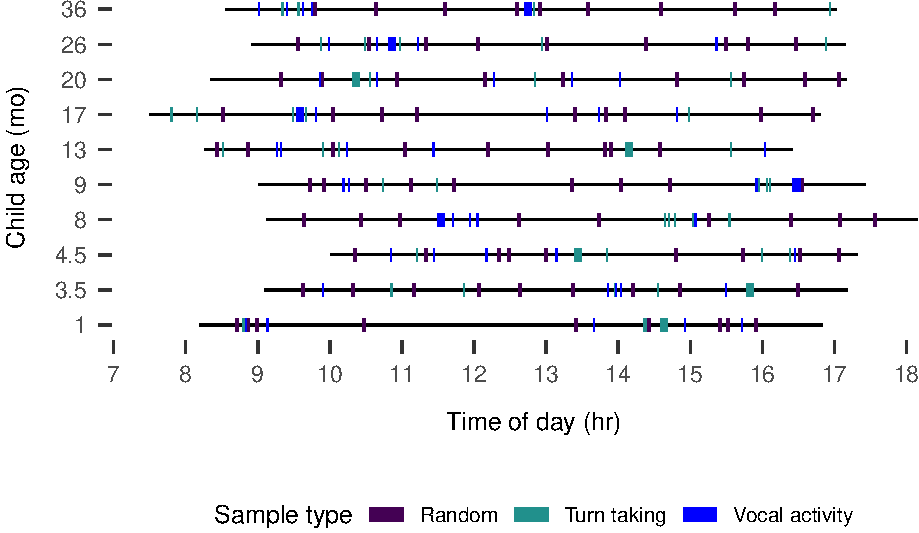
\includegraphics{Yeli-CLE_files/figure-latex/fig1-1.pdf}
\caption{\label{fig:fig1}Recording duration (black line) and sampled clips
(colored boxes) for each of the 10 recordings analyzed, sorted by child
age in months.}
\end{figure}

\subsection{Data selection and annotation}\label{methods-samples}

From the daylong recordings of 57 Rossel children, we selected 10
representative children between ages 0;0 and 3;0 for transcription and
analysis. The 10 children were selected to be spread between the target
age range (0;0--3;0) while also representing a range of typical maternal
education levels found in the community and being evenly split between
male and female children (\protect\hyperlink{tab1}{Table 1}). We
selected a series of non-overlapping sub-clips from each recording for
transcription (\protect\hyperlink{fig1}{Figure 1}) in the following
order: nine randomly-selected 2.5-minute clips, five manually-selected
\enquote{peak} turn-taking activity 1-minute clips, five
manually-selected \enquote{peak} vocal activity 1-minute clips, and one
manually-selected 5-minute expansion of the best one-minute clip, for a
total of 37.5 minutes of transcribed audio for each child (6.25 audio
hours in total). Manual clip selection guidelines are available at . We
annotated limited sub-clips from only 10 children because of the
time-intensive nature of transcribing these naturalistic data; 1 minute
of audio typically took approximately 60--70 minutes to be segmented
into utterances, transcribed, annotated, and loosely translated into
English (\textasciitilde{}400 hours total). Yélî Dnye is almost
exclusively spoken on Rossel Island, where there is no electricity (we
use solar panels) and unreliable access to mobile data, so transcription
was completed over the course of three 4--6 week visits to the island in
2016, 2018, and 2019.

We used the ACLEW Annotation Scheme (Casillas et al., 2017) in ELAN
(Wittenburg, Brugman, Russel, Klassmann, \& Sloetjes, 2006) to
transcribe and annotate all hearable speech in the clips. Using both the
audio and photo context, we segmented out the utterances and ascribed
them to individual speakers (e.g., older brother, mother, aunt, etc.).
We then annotated the vocal maturity of each utterance produced by the
target child (non-canonical babble/canonical babble/single
word/multi-word/unsure) and annotated the addressee of all speech from
other speakers (addressed to the target child/one or more other
children/one or more adults/a mix of adults and children/any
animal/other/unsure). Transcription and annotation was done together by
the first author and one of three community members (all native Yélî
Dnye speakers). The community-based research assistants personally knew
all the families in the recordings, and were able to use their own
experience, the discourse context, and information from the accompanying
photos in reporting what was said and to whom speech was addressed for
each utterance. Detailed manuals and self-guided training materials,
including a \enquote{gold standard test} for this annotation scheme can
be found at .

In what follows we first analyze the nine randomly selected 2.5-minute
clips from each child to establish a baseline view of their speech
environment, focusing on the effects of child age, time of day,
household size, and number of speakers on the rate of target
child-directed (TCDS) and other-directed speech (ODS). Next, we repeat
these analyses, focusing instead only on the turn-taking clips to gain a
view of the speech environment as it appears during the peak
interactions for the day. Then as a first approximation of children's
linguistic development, we map a coarse trajectory of children's use of
babble, first words, and multi-word utterances. Finally, we wrap up by
integrating our Panoramic-approach results with those from prior Close
Study work, relating these findings to the larger literature on
child-directed speech and its role in language development.

\subsection{Statistical models}\label{statistical-models}

We conducted all analyses in R, using the glmmTMB package to run
generalized linear mixed-effects regressions (M. E. Brooks et al., 2017;
R Core Team, 2019) and ggplot2 to generate figures (Wickham, 2016). This
dataset and analysis are available at URL\_MASKED\_FOR\_REVIEW. TCDS and
ODS minutes per hour are naturally restricted to non-negative
(0--infinity) values, causing the distributional variance of those
measures to become positively skewed. To address this issue we use
negative binomial regressions, which can better fit non-negative,
overdispersed data (M. E. Brooks et al., 2017; Smithson \& Merkle,
2013). There were also many cases of zero minutes of TCDS across the
clips---for example, this often occurred in the randomly sampled clips
when the child was sleeping in a quiet area. To handle this additional
distributional characteristic of the data, we added a zero-inflation
model to TCDS analysis which, in addition to the count model of TCDS
(e.g., testing effects of age on the input rate), creates a binary model
to evaluate the likelihood of TCDS being used at all. More conventional,
gaussian linear mixed-effects regressions with log-transformed dependent
variables are provided in the Supplementary Materials, but are
qualitatively similar to what we report here.

\section{Results}\label{results}

The models included the following predictors: child age (months;
centered and standardized), household size (number of people; centered
and standardized), number of non-target-child speakers present in that
clip (centered and standardized), and time of day at the start of the
clip (factor: \enquote{morning} = before 11:00; \enquote{midday} =
11:00--13:00; \enquote{afternoon} = after 13:00). We also included
two-way interactions of (a) child age and the number of speakers present
and (b) child age and time of day, with a random effect of child. For
the zero-inflation model of TCDS, we included the number of speakers
present. We limit our discussion to significant effects; full model
results are provided in the Supplementary Materials.

\begin{figure}
\centering
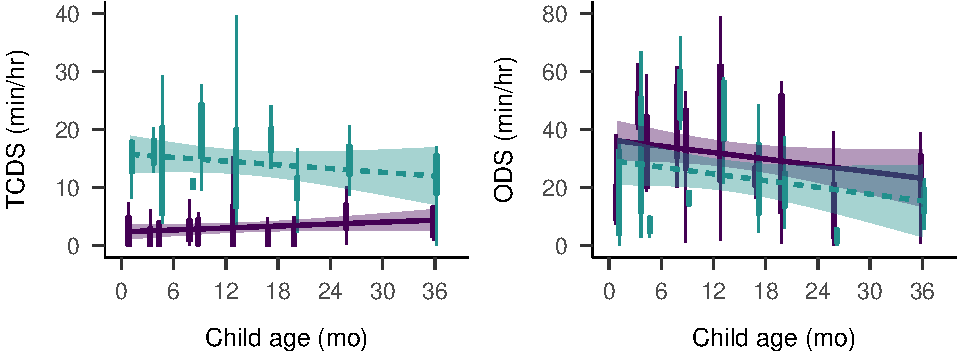
\includegraphics{Yeli-CLE_files/figure-latex/fig2-1.pdf}
\caption{\label{fig:fig2}Estimates of TCDS min/hr (left) and ODS min/hr
(right) across the sampled age range. Each box plot summarizes the data
for one child from the randomly sampled clips (purple; solid) or the
turn taking clips (green; dashed). Bands on the linear trends show 95\%
confidence intervals.}
\end{figure}

\subsection{Target-child-directed speech
(TCDS)}\label{target-child-directed-speech-tcds}

In the random sample, these 10 children heard an average of 3.13 minutes
of speech directly addressed to them per hour (median = 2.95; range =
1.58--6.26; \protect\hyperlink{fig2}{Figure 2} left panel, purple/solid
summaries). For comparison, this is slightly less than reported values
using a near-identical method of data collection, annotation, and
analysis in a Tseltal Mayan community (3.6 minutes per hour for children
under 3;0; Casillas et al. (2019)) and comparable to what has been
reported using a similar method in a Tsimane community (1.6--4.8 minutes
per hour for children under 3;0 depending on what speech is counted;
Scaff et al., in preparation).

The zero-inflated negative binomial regression of TCDS minutes per hour
(N = 90, log-likelihood = -195.26, overdispersion estimate = 3.37)
suggested significant effects of child age, time of day, and their
interaction on the rate at which children are directly addressed. First,
the older children heard a small but significantly greater amount of
TCDS per hour (\protect\hyperlink{fig2}{Figure 2} left panel
purple/solid summaries; B = 0.73, SD = 0.23, z = 3.20, p \textless{}
0.01). Overall, these children were also more likely to hear TCDS in the
mornings (\protect\hyperlink{fig3}{Figure 3} top left panel), with
significantly higher TCDS rates in the morning compared to both midday
(midday-vs-morning: B = 0.80, SD = 0.36, z = 2.23, p = 0.03) and the
afternoon (afternoon-vs-morning: B = 0.54, SD = 0.26, z = 2.10, p =
0.04), and no significant difference in TCDS rate between midday and the
afternoon. However, the time-of-day pattern changed with child age.
Older children were more likely than younger children to show a peak in
TCDS during midday, with a decrease in TCDS between midday and the
afternoon (midday-vs-afternoon: B = -0.60, SD = 0.29, z = -2.04, p =
0.04) and marginally less TCDS in the morning than at midday
(midday-vs-morning: B = -0.59, SD = 0.30, z = -1.94, p = 0.05). There
were no significant effects in either the count or the zero-inflation
models.

Children heard TCDS from a variety of different speakers. Most TCDS came
from adults (mean = 72.65\%, median = 75.51\%, range = 41.41--100\%). On
average, 82.35\% of the total TCDS minutes from adults came from women.
However, an increasing quantity of TCDS with age came from child
speakers (child-TCDS, e.g., from siblings, cousins, or neighbors;
C-TCDS); a Spearman's correlation showed a significant positive
relationship between the average proportion of C-TCDS in a clip and
target child age (Spearman's \emph{rho} = 0.78; \emph{p} = 0.01).

\begin{figure}
\centering
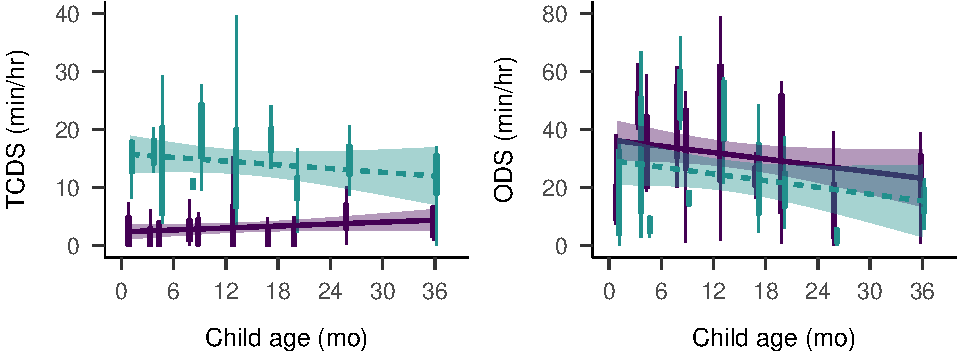
\includegraphics{Yeli-CLE_files/figure-latex/fig3-1.pdf}
\caption{\label{fig:fig3}Estimates of TCDS min/hr (left panels) and ODS
min/hr (right panels) across the recorded day in the random clips (top
panels) and turn-taking (bottom panels) clips. Each box plot summarizes
the data for children age 1;0 and younger (light) or age 1;0 and older
(dark) at the given time of day.}
\end{figure}

\subsection{Other-directed speech
(ODS)}\label{other-directed-speech-ods}

In the random sample, these children heard an average of 35.90 minutes
of other-directed speech per hour (\protect\hyperlink{fig2}{Figure 2}
right panel, purple/solid summaries; median = 32.37; range =
20.20--53.78): that is more than eleven times the average quantity of
speech directed to them, with many clips displaying near-continuous
background speech. For comparison, the prior estimate for Tseltal
children using near-parallel methods found an average of 21 minutes of
overhearable speech per hour (Casillas et al., 2019), and a recent study
of North American children's daylong recordings found that
adult-directed speech (a subset of ODS) occurred at a rate of 7.3
minutes per hour (Bergelson et al., 2019a).

The negative binomial regression of other-directed speech rate (N = 90,
log-likelihood = -370.87, overdispersion estimate = 9.14) revealed
effects of child age, number of speakers present, and time of day on the
rate of ODS encountered. The rate of ODS significantly decreased with
child age (\protect\hyperlink{fig2}{Figure 2} right panel, purple/solid
summaries; B = -0.57, SD = 0.17, z = -3.28, p \textless{} 0.01) and
significantly increased in the presence of more speakers (B = 0.50, SD =
0.05, z = 10.07, p \textless{} 0.001). Across the randomly selected
clips, there were an average of 6.19 speakers present other than the
target child (median = 6; range = 1--19), an average of 59.99\% of whom
were adults. Comparing again to Tseltal and North American English, in
which the average number of speakers present, not including the target
child, was 3.44 and 3.9 respectively (Bergelson et al., 2019a; Casillas
et al., 2019), we can infer that the increased rate of ODS on Rossel
Island is due in part to there simply being more speakers present.
Time-of-day effects on ODS only came through in an interaction with
child age (\protect\hyperlink{fig3}{Figure 3} top right panel). In
particular, older children heard a pattern of ODS mirroring the general
pattern of TCDS; significantly more ODS in the mornings compared to
midday (midday-vs-morning: B = 0.65, SD = 0.20, z = 3.23, p \textless{}
0.01) and the afternoon (afternoon-vs-morning: B = 0.37, SD = 0.15, z =
2.50, p = 0.01). There were no other significant effects on ODS rate.

In sum, the random baseline rates of TCDS and ODS in children's speech
environments are influenced by child age (TCDS increases, ODS
decreases), time of day (both generally peak in the morning), and their
interaction (older children hear more TCDS and less ODS than younger
children at midday). The rate of ODS is also impacted by the number of
speakers present. Correlational results suggest that TCDS comes
increasingly from other children over the first three years. That said,
the baseline rate of TCDS is low, on par with estimates in other
small-scale rural communities (Casillas et al., 2019; Scaff et al., in
preparation), while the ODS rate is quite high relative to estimates in
prior work.

\subsection{TCDS and ODS during interactional
peaks}\label{tcds-and-ods-during-interactional-peaks}

If we instead investigate the rates of TCDS and ODS encountered by these
children during interactional peaks, a different picture emerges
(\protect\hyperlink{fig2}{Figures 2} and \protect\hyperlink{fig3}{3}
green/dashed summaries). The children heard much more TCDS in the
turn-taking clips---14.45 min/hr; more than four times the rate of TCDS
in the random baseline (\protect\hyperlink{fig2}{Figure 2}, left panel,
green/dashed summaries; median = 15.07; range = 9.61--18.73). Children
also heard a reduced rate of ODS: 25.27 min/hr (70.39\% of the
random-sample ODS rate, \protect\hyperlink{fig2}{Figure 2}, right panel,
green/dashed summaries; median = 19.59; range = 6.68--60.18).

The negative binomial mixed-effects regression of TCDS (N = 55,
log-likelihood = -183.25, overdispersion estimate = 2.91) revealed a
significant decrease with child age (B = -0.63, SD = 0.27, z = -2.33, p
= 0.02) and a significant interaction between child age and time of day;
TCDS rate during interactional peaks was marginally higher for older
children at morning compared to midday (midday-vs-morning: B = 0.53, SD
= 0.28, z = 1.89, p = 0.06) and significantly higher in the afternoon
than at midday (midday-vs-afternoon: B = 0.61, SD = 0.28, z = 2.17, p =
0.03; see \protect\hyperlink{fig3}{Figure 3}, bottom left panel).

As in the random sample, an increasing portion of TCDS during
interactional peaks came from other children with age. While, overall,
more of the TCDS in interactional peaks came from adults than in the
random clips (mean = 82.68\%, median = 88.04\%, range = 50--100\%), a
Spearman's correlation showed an even stronger positive relationship
between the average proportion of child TCDS in a clip and target child
age (Spearman's \emph{rho} = 0.92; \emph{p} = \textless{} 0.001).
Notably, women contributed proportionally less TCDS during interactional
peaks than they did during the random clips: on average, women
contributed 61.55\% of the children's TCDS minutes from adults in the
turn-taking clips (compared to 82.35\% in the random clips). In brief,
compared to the random sample, interactional peaks included more
directed speech from men and, for older target children, more directed
speech from other children.

The negative binomial mixed-effects regression of ODS (N = 55,
log-likelihood = -202.60, overdispersion estimate = 4.66) only revealed
a significant effect of number of speakers. As before, ODS rates were
higher when more speakers were present (B = 0.56, SD = 0.08, z = 6.76, p
\textless{} 0.001). There were no other significant effects on ODS rate
(\protect\hyperlink{fig3}{Figure 3}, bottom right panel).

Overall, the results suggest that these children typically hear very
little directly addressed speech, but that interactional peaks provide
opportunities for dense input. While the majority of directed speech
comes from women, an increasing portion of it comes from other children
with age, and directed speech from men is more likely during
interactional peaks. Directed and overhearable speech are most likely to
occur during the morning, before most of the household has dispersed for
their work activities, similar to other findings from subsistence
farming households (Casillas et al., 2019). However, older children are
more likely than younger children to show higher input rates at midday,
perhaps due to their increased interactions with other children while
adults attend to gardening and domestic tasks. Possibly because of the
large number of speakers present, these children were also in the
vicinity of voluminous overhearable speech, underscoring the
availability of other-addressed speech as a resource for linguistic
input in this context.

\subsection{Vocal maturity}\label{vocal-maturity}

Given the low baseline rate of directed speech, one might expect that
Rossel children's early linguistic development, particularly the onset
and use of single- and multi-word utterances, shows delays in comparison
to children growing up in more CDS-rich environments. We plotted the
proportion of all linguistic vocalizations for each child (i.e.,
discarding laughter, crying, or unknown-types; leaving a total of 4308
vocalizations) that fell into the following categories: non-canonical
babble, canonical babble, single-word utterance, or multi-word
utterance. Children are expected to traverse all four types of
vocalization during development such that they primarily produce single-
and multi-word utterances by age three.

In the onset of use for canonical babble, first words, and multi-word
utterances, these Rossel children's vocalization data closely resemble
expectations based on populations of children who hear more CDS
(\protect\hyperlink{fig4}{Figure 4}). Canonical babble appears in the
second half of the first year, first words appear around the first
birthday, and multi-word utterances appear a few months after that
(Frank et al., in preparation; Kuhl, 2004; Pine \& Lieven, 1993; Slobin,
1970; Tomasello \& Brooks, 1999; Warlaumont, Richards, Gilkerson, \&
Oller, 2014). Rossel children also far exceeded the canonical babbling
ratio (CBR) associated with major developmental delay (proportional use
of speech-like vocalizations \textgreater{} 0.15 by 0;10; Cychosz et
al., under reviewa; Oller, Eilers, Basinger, Steffens, \& Urbano, 1995);
the minimum CBR among Rossel children 0;9 and older was 0.22 (mean =
0.63; median = 0.68; range = 0.22--0.86).

Over all annotated clips, children produced an average of 7.18
linguistic vocalizations per minute (median = 7.79; range = 4.57--8.95),
less frequently than children in short recordings of American
infant-caregiver interaction (Oller et al., 1995) but similar to
estimates for Tseltal children (Brown, 2011; Casillas et al., 2019).

\begin{figure}
\centering
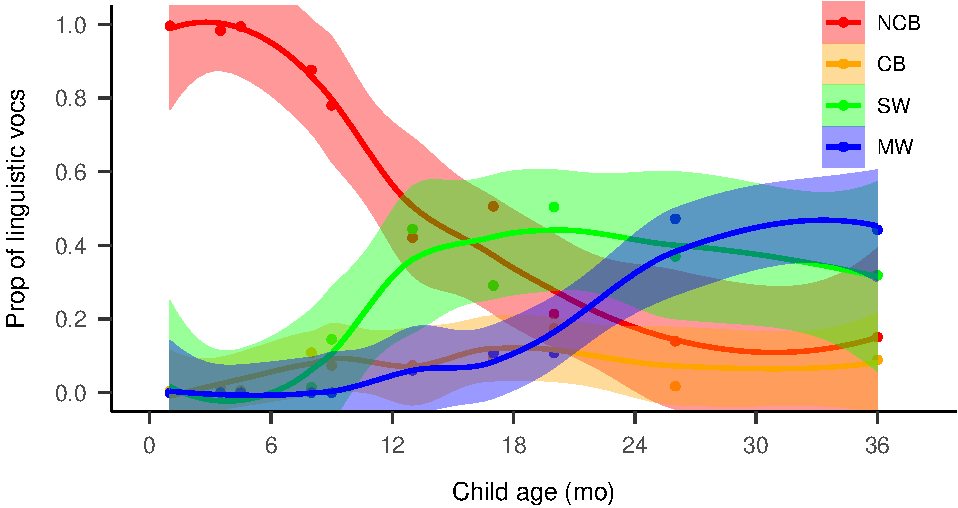
\includegraphics{Yeli-CLE_files/figure-latex/fig4-1.pdf}
\caption{\label{fig:fig4}Proportion of vocalization types used by children
across age (NCB = Non-canonical babble, CB = Canonical babble, SW =
single word utterance, MW = multi-word utterance).}
\end{figure}

\section{Discussion}\label{disc}

We analyzed the speech environments of 10 Rossel children under age 3;0
to investigate: (a) how often children were spoken to directly, (b) how
much other overhearable speech is available to them, (c) how these
sources of linguistic input are shaped by child age and interactional
context, and (d) whether this (relatively) low rate of directed input
appears to impact their early production milestones.

Based on prior ethnographic work, we expected that these children would
hear frequent child-directed speech from a wide variety of caregivers
and frequent speech directed to others (Brown \& Casillas, in press). In
fact, in these daylong audio recordings, children were rarely directly
addressed. This low baseline rate of TCDS is comparable to that found in
a Tseltal community where minimal TCDS is one means to socializing
children into attending to their surroundings. On the other hand, the
Rossel child speech environment contains ample overhearable speech; much
more than has been reported elswhere, at time of writing. The low
relative rate of TCDS and the high incidence of ODS may be partly
attributable to the fact that several speakers are typically present
across the day, as discussed further below.

Prior work also led us to expect that the quantity of TCDS would be
stable across the age range studied (Bergelson et al., 2019b; Casillas
et al., 2019; Scaff et al., in preparation), and that an increasing
proportion of it would come from other children (Brown, 2011; Brown \&
Casillas, in press; Shneidman \& Goldin-Meadow, 2012). Counter to
expectations, we found a small but significant increase in TCDS rate
with child age in the random clips and a small and significant
\emph{decrease} in TCDS rate with age in the turn-taking clips. The
age-related baseline increase in TCDS may derive from more frequent
participation in independent play with other children; in prior work,
increased proportional input from other children was also associated
with an increase in overall input rate (Shneidman \& Goldin-Meadow,
2012). The age-related decrease in TCDS rate during peak interactional
moments was not expected, but may be attributable to this change in
interactional partners with age; if adults are more likely to be the
source of TCDS during interactional peaks for younger children, they may
also provide more voluminous speech during those peaks than other
children do during interactional peaks later in development. Sleep
during the day may also help explain these patterns; if older children
sleep less than younger children, they may be more likely hear more TCDS
during random but not peak-based clips. All of these explanations
require follow-up work from a larger sample of children and, ideally,
from a larger sample of their interactions throughout the day. ODS
decreased with age, consistent with prior Panoramic studies with both
Western and non-Western samples (Bergelson et al., 2019b; Casillas et
al., 2019; Scaff et al., in preparation).

Finally, while we anticipated that the children's input would be
non-uniformly distributed over the recording day (Abney et al., 2017;
Casillas et al., 2019), we also expected to see a somewhat more even
distribution of directed speech from morning to evening. Young Rossel
children have been reported to pass between multiple caregivers during a
typical day. We expected that this care-sharing practice might weaken
the effect of farming activities on linguistic input rate, found in the
late morning and early afternoon in previous work with Tseltal Mayan
subsistence farmers (Casillas et al., 2019). In fact, we found that
children's rate of linguistic input was still significantly impacted by
time of day, similar to the Tseltal farmers: most TCDS and ODS came
during the morning, with older children more likely to hear TCDS at
midday than younger children, possibly because midday is when most
adults are likely attending to other duties while children congregate in
large play groups.

\subsection{Diverging Close Study and Panoramic
perspectives}\label{diverging-close-study-and-panoramic-perspectives}

We predicted that infants on Rossel Island would hear more frequent
directed speech than has been found in other subsistence farming
contexts (e.g., Brown, 2011, 2014; Brown \& Casillas, in press; Casillas
et al., 2019; de León, 2000; Frye, 2019; Ochs \& Schieffelin, 1984; Pye,
1986; Rumsey, San Roque, \& Schieffelin, 2013). We made this prediction
on the basis of two prior ethnographic observations (see Brown \&
Casillas (in press) for details). First, Rossel adults and children have
been shown to talk to children, even young infants, as if they can
understand and respond to what is being said. Second, infants and young
children often traverse a wide network of caregivers who are available
to interact with them for some period. Our Panoramic findings, based on
daylong audio data from 10 children, differ from these expectations:
there is minimal TCDS to young children, time of day strongly impacts
the rate of linguistic input, and there is limited variability in the
type of speakers typically talking to children.

We found that the 10 Rossel children here heard slightly less TCDS than
was documented for the Tseltal children. Taking the Mayan and Papuan
findings together, we suggest that the Panoramic approach is not
effective for distinguishing distinct caregiver attitudes toward talking
to young children. While Rossel caregivers view their children, even
their young infants, as potential co-interactants in conversational play
(Brown \& Casillas, in press), the circumstances of everyday life shape
the children's broader linguistic landscape such that most of what
children hear is talk between others. We suggest that, in the daylong
context, caregivers from these two subsistence farming communities are
preoccupied for most of the day with social and domestic commitments in
which they are motivated to converse with the other adults and (older)
children present; not just to get their daily tasks done but also
because these more mature speakers enable more complex verbal
interactions and social routines. Given the multi-generational and
patrilocal settlement patterns in both communities, there are frequent
opportunities to engage with other adults and older children. This same
explanation extends to the variability in linguistic input encountered
by children over the day and from different speaker types; rather than
being passed between caregivers who are \enquote{available} to interact
with them, young children may accompany their varied caregivers in their
shared daily tasks, switching from lap to lap without the activity
context necessarily changing.

When it comes to quantifying how much linguistic input children
encounter, the Panoramic view yields the important insight that direct
linguistic input is rare on average; it exists primarily during short
interactional peaks. We suspect that it is during these interactional
peaks that caregiver attitudes about how to engage children in
interaction are most clearly expressed. Indeed it is during
interactional peaks when we see not only more TCDS but also TCDS from
more diverse speaker types. In contrast, the randomly sampled Panoramic
data demonstrate how the number of speakers present and the routines of
everyday life strongly shape the overall rate of linguistic input
available in children's environments. That is, the forces shaping the
rate of Rossel children's linguistic input are somewhat different from
the forces shaping the content and sources of their linguistic input.
This insight is critical in trying to join cognitive and social models
of children's early language development. After all,
children---particularly children in contexts with minimal TCDS---may do
most of their language learning during these short bursts in the day
when they are jointly attending to language during interactions with
others. If so, it would be more efficient to aim models of learning and
annotation time at these interactional peaks. Indeed, such a hybrid
approach may be optimal for accessing varied, ecologically valid,
culturally distinct codes of verbal interaction while also sketching a
stable picture of early language exposure specific to those same
communities (Shneidman, 2010; Shneidman \& Goldin-Meadow, 2012). Further
cross-cultural work on children's ability to learn from massed
vs.~distributed and directed vs.~overhearable language use (e.g.,
Akhtar, Jipson, \& Callanan, 2001; Schwab \& Lew-Williams, 2016) is a
critical route for further investigation into how these sources of
linguistic input may be leveraged for language development.

\subsection{Independence and
child-TCDS}\label{independence-and-child-tcds}

The increase in TCDS from other children in this Rossel data recalls
findings from Shneidman and Goldin-Meadow (2012) in which Yucatec Mayan
children's directed speech rate increased enormously between ages one
and three, primarily due to increased input from other children. We saw
a significant, but much smaller overall increase in TCDS in these 10
Rossel children's recordings, with an increasing proportion of that
input coming from children. Interestingly, prior work with a Tseltal
community---culturally more proximal to the Yucatec families studied in
Shneidman and Goldin-Meadow (2012)---found no evidence for increased
input from other children in this same age range (0;0--3;0; Casillas et
al., 2019). The lack of child TCDS in the study of Tseltal Mayan
children was attributed to the observation that they only begin to
engage in independent, extended play with other children \emph{after}
age three. In comparison, prior ethnographic work on Rossel Island
highlights independence as a primary concern for parents of young
children; from early toddlerhood Rossel children are encouraged to
choose how they dress, when and what to eat, and who to visit (Brown \&
Casillas, in press). The formation of hamlets in a cluster around a
shared open area, often close to a shallow swimming area, further
nurtures a sense of safe, free space in which children can wander. These
features of childhood on Rossel Island support extended independent play
with other children from an early age and may help explain the strongly
increasing presence of child TCDS in the present data. Further work
combining the time of day and interlocutor effects found here with
ethnographic interview data are needed to explore these ideas in full.
Overall, we see that children's linguistic input shifts in the first
three years, with proportionally more speech coming from less mature
talkers; how this influences their early linguistic development,
particularly given the minimal overall rate of TCDS, is open to further
research.

\subsection{Trade-offs in the use of Panoramic
methods}\label{trade-offs-in-the-use-of-panoramic-methods}

The present study used Panoramic methods to get a broader view of 10
Rossel children's linguistic landscapes, but was limited in both the
number of children represented and the number of annotated minutes
analyzed per child. The data presented here, though transcribed, were
only analyzed for superficial features of children's linguistic
environment: input rates of directed and overhearable speech and
children's vocal maturity. A Close Study approach is needed in order to
make semantically rich interpretations of what children are saying and
hearing or to delineate cross-cultural differences in the content or
style of child-directed speech.

While our Panoramic approach effectively captured circumstantial
variation over the course of a waking day, it did \emph{not} completely
avoid the Observer's Paradox (Labov, 1972); upon transcribing the data
we found both moments when the speakers seemed to ignore the recorder
and moments when it was the focus of discussion. The latter case often
arose when new interactants came into contact with the child---a
relatively frequent event---prompting the caregiver to explain and warn
about the devices. There was also at least one case when a mother
reported that the father, who is typically at home, avoided our recorder
by spending the entire day elsewhere. Daylong methods then may decrease
the intensity and continuity of the Observer's Paradox, but do not
eliminate it entirely. With this in mind, close ethnographic work over a
longer period with a handful of families may, in fact, be the optimal
way to minimize these effects. However, this approach severely limits
the possible sample size of a study. What, then, is the ideal approach
for exploring the variable linguistic environments in which children are
raised?

When it comes to drawing inferences about the deeper forces shaping
caregiver-child interaction and how they vary across cultures or, for
that matter, any other task that requires researchers to grapple with
what is actually \emph{meant} during interaction, a Close Study approach
is the only real option. Even when applying a microanalytic approach to
short clips derived from daylong recordings, the researcher likely will
lack sufficient visual and interactional context to adequately
reconstruct the scene. In this use case, short recordings maintain an
advantage, particularly when Observer Paradox effects can be reduced by
investing significant time with each observed family (e.g., over a
high-density longitudinal study).

However, when it comes to quantifying the use of linguistic features in
order to explore the feasibility of specific learning mechanisms (e.g.,
CDS as a facilitatory context for referential word learning), daylong
data are crucial for establishing the frequency and circumstances under
which the critical linguistic or interactional \enquote{data} are
encountered. Given our present findings and those of Casillas et al.
(2019), studies focused on particular linguistic features of CDS (e.g.,
relative use of certain syntactic structures) may benefit from focusing
annotation time on interactional peaks---where these features are much
more likely to be on display---with less time dedicated to establishing
a baseline estimate of CDS frequency (see also Bergelson et al.
(2019a)). Importantly, researchers making daylong recordings in a
context where they are a cultural outsider should always do their
recording collection in parallel with or following some ethnographic
work to avoid the serious and potentially harmful pitfalls discussed in
the Introduction (see also Cychosz et al. (acceptedb)).

We propose that the most promising long-term approach for using input
patterns to test the feasibility of individual learning mechanisms is to
strategically sub-sample daylong recordings made with a representative
participant sample of the community studied, while maintaining
comparable speech environment measures across communities whenever
possible. This approach is suitable for tracking variation among related
but distinct ethnolinguistic populations, which can help disentangle
input and development effects related to the specific linguistic and
cultural context in which each child is raised (as proposed by Pye
(2017); or a diversity-centric approach, as in Moran, Schikowski,
Pajović, Hysi, and Stoll (2016)), maintaining comparable speech
environment measures whenever possible. The current study pales in
comparison to this ideal, but hope to see this vision realized in future
work.

\subsection{Conclusion}\label{disc-conclusion}

We estimate that, on average, children on Rossel Island under age 3;0
hear 3.13 minutes of directed speech per hour, with an average of 14.45
minutes per hour during peak interactive moments during the day. Most of
directed speech comes from adults, but older children hear more directed
speech from other children. There is also an average 35.90 minutes per
hour of overhearable speech present. Older children heard more directed
speech and less overhearable speech than younger children. Bursts of
speech featuring mostly TCDS appear to be present from infancy onward.
Despite this relatively low rate of directed speech, these children's
vocal maturity appears on-track with norms for typically developing
children in multiple diverse populations (Cychosz et al., under reviewa;
Lee, Jhang, Relyea, Chen, \& Oller, 2018; Warlaumont et al., 2014).

Our findings diverged in several ways from expectations developed on the
basis of prior ethnographic work in this community, including the
frequency of child-directed talk, the diversity of talkers, and the
distribution of talk over the course of the day. When considered
together with data from a Mayan community, the findings suggest that the
Panoramic approach, while well suited to gathering inclusive,
ecologically valid estimates of how much linguistic input children hear,
is also far more sensitive to circumstantial variation (e.g., the number
of speakers present) than it is to established ideological variation in
how caregivers talk to children. For the latter, a Close Study or other
hybrid approach is needed (e.g., analyzing content in interactional
peaks). Whether child language development is better predicted by
meaningful individual differences in average circumstantial variation
(e.g., Panoramic input quantity), ideologically-based variation (e.g.,
attitudes toward language pedagogy), or something inbetween is a
question for future work. Cross-cultural and cross-linguistic data will
have a major role to play in teasing out the causal factors at play in
this larger issue relating children's early linguistic experience to
their later language development.

Importantly, the data presented here come from an evolving corpus of
Yélî Dnye developmental data; any reader interested in citing
descriptive features of the Rossel child language environment is
strongly encouraged to visit the following address for up-to-date
estimates: URL\_MASKED\_FOR\_REVIEW. The information on that linked page
will include any new data, annotations, and analyses added after the
publication of this study.

\section{Acknowledgements}\label{acknowledgements}

\newpage

\section{References}\label{refs}

\begingroup
\setlength{\parindent}{-0.5in} \setlength{\leftskip}{0.5in}

\hypertarget{refs}{}
\hypertarget{ref-abney2017time}{}
Abney, D. H., Smith, L. B., \& Yu, C. (2017). It's time: Quantifying the
relevant time scales for joint attention. In G. Gunzelmann, A. Howes, T.
Tenbrink, \& E. Davelaar (Eds.), \emph{Proceedings of the 39th Annual
Meeting of the Cognitive Science Society} (pp. 1489--1494). London, UK.

\hypertarget{ref-akhtar2001learning}{}
Akhtar, N., Jipson, J., \& Callanan, M. A. (2001). Learning words
through overhearing. \emph{Child Development}, \emph{72}(2), 416--430.

\hypertarget{ref-anderson2019modeling}{}
Anderson, H., \& Fausey, C. (2019). Modeling nonuniformities in infants'
everyday speech environments. presented at the biennial meeting of the
society for research on child development. baltimore, md.

\hypertarget{ref-bates1997inseparability}{}
Bates, E., \& Goodman, J. C. (1997). On the inseparability of grammar
and the lexicon: Evidence from acquisition, aphasia, and real-time
processing. \emph{Language and Cognitive Processes}, \emph{12}(5--6),
507--584.
doi:\href{https://doi.org/10.1080/016909697386628}{10.1080/016909697386628}

\hypertarget{ref-bergelsonIPbsl}{}
Bergelson, E., Alphen, P. van, Benneti, L., Bunce, J., Casillas, M.,
Guez, A., \ldots{} Cristia, A. (in preparation). Child language
environments in \textgreater{}2500 daylong recordings across 5
continents.

\hypertarget{ref-bergelson2019day}{}
Bergelson, E., Amatuni, A., Dailey, S., Koorathota, S., \& Tor, S.
(2019a). Day by day, hour by hour: Naturalistic language input to
infants. \emph{Developmental Science}, \emph{22}(1), e12715.
doi:\href{https://doi.org/10.1111/desc.12715}{10.1111/desc.12715}

\hypertarget{ref-bergelsoncasillas2019what}{}
Bergelson, E., Casillas, M., Soderstrom, M., Seidl, A., Warlaumont, A.
S., \& Amatuni, A. (2019b). What do North American babies hear? A
large-scale cross-corpus analysis. \emph{Developmental Science},
\emph{22}(1), e12724.
doi:\href{https://doi.org/10.1111/desc.12724}{10.1111/desc.12724}

\hypertarget{ref-brinchmann2019direct}{}
Brinchmann, E. I., Braeken, J., \& Lyster, S.-A. H. (2019). Is there a
direct relation between the development of vocabulary and grammar?
\emph{Developmental Science}, \emph{22}(1), e12709.
doi:\href{https://doi.org/10.1111/desc.12709}{10.1111/desc.12709}

\hypertarget{ref-brooks2017modeling}{}
Brooks, M. E., Kristensen, K., van Benthem, K. J., Magnusson, A., Berg,
C. W., Nielsen, A., \ldots{} Bolker, B. M. (2017). Modeling
zero-inflated count data with glmmTMB. \emph{bioRxiv}.
doi:\href{https://doi.org/10.1101/132753}{10.1101/132753}

\hypertarget{ref-brown2011cultural}{}
Brown, P. (2011). The cultural organization of attention. In A. Duranti,
E. Ochs, \& and B. B. Schieffelin (Eds.), \emph{Handbook of Language
Socialization} (pp. 29--55). Malden, MA: Wiley-Blackwell.

\hypertarget{ref-brown2014interactional}{}
Brown, P. (2014). The interactional context of language learning in
Tzeltal. In I. Arnon, M. Casillas, C. Kurumada, \& B. Estigarribia
(Eds.), \emph{Language in interaction: Studies in honor of Eve V. Clark}
(pp. 51--82). Amsterdam, NL: John Benjamins.

\hypertarget{ref-brownIPchildrearing}{}
Brown, P., \& Casillas, M. (in press). Childrearing through social
interaction on Rossel Island, PNG. In A. J. Fentiman \& M. Goody (Eds.),
\emph{Esther Goody revisited: Exploring the legacy of an original
inter-disciplinarian} (pp. XX--XX). New York, NY: Berghahn.

\hypertarget{ref-brown2014language}{}
Brown, P., \& Gaskins, S. (2014). Language acquisition and language
socialization. In N. J. Enfield, P. Kockelman, \& J. Sidnell (Eds.),
\emph{Handbook of Linguistic Anthropology} (pp. 187--226). Cambridge,
UK: Cambridge University Press.
doi:\href{https://doi.org/10.1017/CBO9781139342872.010}{10.1017/CBO9781139342872.010}

\hypertarget{ref-cartmill2013quality}{}
Cartmill, E. A., Armstrong, B. F., Gleitman, L. R., Goldin-Meadow, S.,
Medina, T. N., \& Trueswell, J. C. (2013). Quality of early parent input
predicts child vocabulary 3 years later. \emph{Proceedings of the
National Academy of Sciences}, \emph{110}(28), 11278--11283.
doi:\href{https://doi.org/10.1073/pnas.1309518110}{10.1073/pnas.1309518110}

\hypertarget{ref-casillas2019stepbystep}{}
Casillas, M., \& Cristia, A. (2019). A step-by-step guide to collecting
and analyzing long-format speech environment (lfse) recordings.
\emph{Collabra: Psychology}, \emph{5}(1), 24.
doi:\href{https://doi.org/10.1525/collabra.209}{10.1525/collabra.209}

\hypertarget{ref-casillas2019early}{}
Casillas, M., Brown, P., \& Levinson, S. C. (2019). Early language
experience in a tseltal mayan village. \emph{Child Development},
\emph{OnlineOpen}(X), XX--XX.

\hypertarget{ref-casillas2017ACLEWDAS}{}
Casillas, M., Bunce, J., Soderstrom, M., Rosemberg, C., Migdalek, M.,
Alam, F., \ldots{} Garrison, H. (2017). Introduction: The ACLEW DAS
template {[}training materials{]}. Retrieved from
\url{https://osf.io/aknjv/}

\hypertarget{ref-cychoszURcanonical}{}
Cychosz, M., Cristia, A., Bergelson, E., Casillas, M., Baudet, G.,
Warlaumont, A. S., \ldots{} Seidl, A. (under reviewa). Canonical babble
development in a large-scale crosslinguistic corpus. Retrieved from
\url{https://osf.io/ca6qu/}

\hypertarget{ref-cychoszURlongform}{}
Cychosz, M., Romeo, R., Soderstrom, M., Scaff, C., Ganek, H., Cristia,
A., \ldots{} Weisleder, A. (acceptedb). Longform recordings of everyday
life: Ethics for best practices.

\hypertarget{ref-deleon2000emergent}{}
de León, L. (2000). The emergent participant: Interactive patterns in
the socialization of Tzotzil (Mayan) infants. \emph{Journal of
Linguistic Anthropology}, \emph{8}(2), 131--161.

\hypertarget{ref-deleon2011language}{}
de León, L. (2011). Language socialization and multiparty participation
frameworks. In A. Duranti, E. Ochs, \& and B. B. Schieffelin (Eds.),
\emph{Handbook of Language Socialization} (pp. 81--111). Malden, MA:
Wiley-Blackwell.
doi:\href{https://doi.org/10.1002/9781444342901.ch4}{10.1002/9781444342901.ch4}

\hypertarget{ref-frankIPvariability}{}
Frank, M. C., Braginsky, M., Marchman, V. A., \& Yurovsky, D. (in
preparation). \emph{Variability and consistency in early language
learning: The Wordbank project}. Retrieved from
\url{https://langcog.github.io/wordbank-book/}

\hypertarget{ref-frye2019thesis}{}
Frye, H. (2019). \emph{Child directed speech in Qaqet} (PhD thesis).
University of Cologne.

\hypertarget{ref-gaskins2000childrens}{}
Gaskins, S. (2000). Children's daily activities in a Mayan village: A
culturally grounded description. \emph{Cross-Cultural Research},
\emph{34}(4), 375--389.
doi:\href{https://doi.org/10.1177/106939710003400405}{10.1177/106939710003400405}

\hypertarget{ref-gaskins2006cultural}{}
Gaskins, S. (2006). Cultural perspectives on infant--caregiver
interaction. In N. J. Enfield \& S. Levinson (Eds.), \emph{Roots of
Human Sociality: Culture, Cognition and Interaction} (pp. 279--298).
Oxford: Berg.

\hypertarget{ref-hart1995meaningful}{}
Hart, B., \& Risley, T. R. (1995). \emph{Meaningful Differences in the
Everyday Experience of Young American Children}. Paul H. Brookes
Publishing.

\hypertarget{ref-hoff2003specificity}{}
Hoff, E. (2003). The specificity of environmental influence:
Socioeconomic status affects early vocabulary development via maternal
speech. \emph{Child Development}, \emph{74}(5), 1368--1378.
doi:\href{https://doi.org/10.3389/fpsyg.2015.01492}{10.3389/fpsyg.2015.01492}

\hypertarget{ref-hurtado2008does}{}
Hurtado, N., Marchman, V. A., \& Fernald, A. (2008). Does input
influence uptake? Links between maternal talk, processing speed and
vocabulary size in spanish-learning children. \emph{Developmental
Science}, \emph{11}(6), F31--F39.

\hypertarget{ref-huttenlocher2010sources}{}
Huttenlocher, J., Waterfall, H., Vasilyeva, M., Vevea, J., \& Hedges, L.
V. (2010). Sources of variability in children's language growth.
\emph{Cognitive Psychology}, \emph{61}(4), 343--365.
doi:\href{https://doi.org/10.1016/j.cogpsych.2010.08.002}{10.1016/j.cogpsych.2010.08.002}

\hypertarget{ref-kuhl2004early}{}
Kuhl, P. K. (2004). Early language acquisition: Cracking the speech
code. \emph{Nature Reviews Neuroscience}, \emph{5}(11), 831.
doi:\href{https://doi.org/10.1038/nrn1533}{10.1038/nrn1533}

\hypertarget{ref-labov1972sociolinguistic}{}
Labov, W. (1972). \emph{Sociolinguistic patterns}. Philadelphia:
University of Pennsylvania.

\hypertarget{ref-lee2018babbling}{}
Lee, C.-C., Jhang, Y., Relyea, G., Chen, L.-m., \& Oller, D. K. (2018).
Babbling development as seen in canonical babbling ratios: A
naturalistic evaluation of all-day recordings. \emph{Infant Behavior and
Development}, \emph{50}, 140--153.

\hypertarget{ref-lieven1997lexically}{}
Lieven, E. V. M., Pine, J. M., \& Baldwin, G. (1997). Lexically-based
learning and early grammatical development. \emph{Journal of Child
Language}, \emph{24}(1), 187--219.
doi:\href{https://doi.org/10.1017/S0305000996002930}{10.1017/S0305000996002930}

\hypertarget{ref-marchman2004language}{}
Marchman, V. A., Martínez-Sussmann, C., \& Dale, P. S. (2004). The
language-specific nature of grammatical development: Evidence from
bilingual language learners. \emph{Developmental Science}, \emph{7}(2),
212--224.
doi:\href{https://doi.org/10.1111/j.1467-7687.2004.00340.x}{10.1111/j.1467-7687.2004.00340.x}

\hypertarget{ref-moran2016acqdiv}{}
Moran, S., Schikowski, R., Pajović, D., Hysi, C., \& Stoll, S. (2016).
The acqdiv database: Min(d)ing the ambient language. In
\emph{Proceedings of the tenth international conference on language
resources and evaluation (lrec 2016)} (pp. 4423--4429). Portorož,
Slovenia.

\hypertarget{ref-ochs1984language}{}
Ochs, E., \& Schieffelin, B. (1984). Language acquisition and
socialization: Three developmental stories and their implications. In R.
A. Schweder \& R. A. LeVine (Eds.), \emph{Culture theory: Essays on
mind, self, and emotion} (pp. 276--322). Cambridge University Press.

\hypertarget{ref-oller1995extreme}{}
Oller, D. K., Eilers, R. E., Basinger, D., Steffens, M. L., \& Urbano,
R. (1995). Extreme poverty and the development of precursors to the
speech capacity. \emph{First Language}, \emph{15}(44), 167--187.

\hypertarget{ref-pine1993reanalysing}{}
Pine, J. M., \& Lieven, E. V. M. (1993). Reanalysing rote-learned
phrases: Individual differences in the transition to multi-word speech.
\emph{Journal of Child Language}, \emph{20}(3), 551--571.
doi:\href{https://doi.org/10.1017/S0305000900008473}{10.1017/S0305000900008473}

\hypertarget{ref-pye1986quiche}{}
Pye, C. (1986). Quiché Mayan speech to children. \emph{Journal of Child
Language}, \emph{13}(1), 85--100.
doi:\href{https://doi.org/10.1017/S0305000900000313}{10.1017/S0305000900000313}

\hypertarget{ref-pye2017comparative}{}
Pye, C. (2017). \emph{The Comparative Method of Language Acquisition
Research}. University of Chicago Press.

\hypertarget{ref-R-base}{}
R Core Team. (2019). \emph{R: A language and environment for statistical
computing}. Vienna, Austria: R Foundation for Statistical Computing.
Retrieved from \url{https://www.R-project.org/}

\hypertarget{ref-rogoff2003firsthand}{}
Rogoff, B., Paradise, R., Arauz, R. M., Correa-Chávez, M., \& Angelillo,
C. (2003). Firsthand learning through intent participation. \emph{Annual
Review of Psychology}, \emph{54}(1), 175--203.
doi:\href{https://doi.org/10.1146/annurev.psych.54.101601.145118}{10.1146/annurev.psych.54.101601.145118}

\hypertarget{ref-rowe2008child}{}
Rowe, M. L. (2008). Child-directed speech: Relation to socioeconomic
status, knowledge of child development and child vocabulary skill.
\emph{Journal of Child Language}, \emph{35}(1), 185--205.
doi:\href{https://doi.org/10.1017/S0305000907008343}{10.1017/S0305000907008343}

\hypertarget{ref-rumsey2013ergative}{}
Rumsey, A., San Roque, L., \& Schieffelin, B. B. (2013). The acquisition
of ergative marking in Kaluli, Ku Waru and Duna (Trans New Guinea). In
E. L. Bavin \& S. Stoll (Eds.), \emph{Sabine} (pp. 139--188). Amsterdam;
New York: John Benjamins Publishing Company.

\hypertarget{ref-scaffIPlanguage}{}
Scaff, C., Stieglitz, J., Casillas, M., \& Cristia, A. (in preparation).
Language input in a hunter-forager population: Estimations from daylong
recordings.

\hypertarget{ref-schwab2016repetition}{}
Schwab, J. F., \& Lew-Williams, C. (2016). Repetition across successive
sentences facilitates young children's word learning.
\emph{Developmental Psychology}, \emph{52}(6), 879--886.
doi:\href{https://doi.org/10.1037/dev0000125}{10.1037/dev0000125}

\hypertarget{ref-shneidman2010language}{}
Shneidman, L. A. (2010). \emph{Language Input and Acquisition in a Mayan
Village} (PhD thesis). The University of Chicago.

\hypertarget{ref-shneidman2012language}{}
Shneidman, L. A., \& Goldin-Meadow, S. (2012). Language input and
acquisition in a Mayan village: How important is directed speech?
\emph{Developmental Science}, \emph{15}(5), 659--673.
doi:\href{https://doi.org/10.1111/j.1467-7687.2012.01168.x}{10.1111/j.1467-7687.2012.01168.x}

\hypertarget{ref-slobin1970universals}{}
Slobin, D. I. (1970). Universals of grammatical development in children.
In G. B. Flores d'Arcais \& W. J. M. Levelt (Eds.), \emph{Advances in
Psycholinguistics} (pp. 174--186). Amsterdam, NL: North Holland
Publishing.

\hypertarget{ref-smithson2013generalized}{}
Smithson, M., \& Merkle, E. (2013). \emph{Generalized linear models for
categorical and continuous limited dependent variables}. New York:
Chapman; Hall/CRC.
doi:\href{https://doi.org/10.1201/b15694}{10.1201/b15694}

\hypertarget{ref-tamislemonda2017power}{}
Tamis-LeMonda, C. S., Kuchirko, Y., Luo, R., Escobar, K., \& Bornstein,
M. H. (2017). Power in methods: Language to infants in structured and
naturalistic contexts. \emph{Developmental Science}, \emph{20}(6),
e12456.
doi:\href{https://doi.org/10.1111/desc.12456}{10.1111/desc.12456}

\hypertarget{ref-tomasello1999early}{}
Tomasello, M., \& Brooks, P. J. (1999). Early syntactic development: A
Construction Grammar approach. In M. Barrett (Ed.), \emph{The
Development of Language} (pp. 161--190). New York: Psychology Press.

\hypertarget{ref-warlaumont2014social}{}
Warlaumont, A. S., Richards, J. A., Gilkerson, J., \& Oller, D. K.
(2014). A social feedback loop for speech development and its reduction
in Autism. \emph{Psychological Science}, \emph{25}(7), 1314--1324.
doi:\href{https://doi.org/10.1177/0956797614531023}{10.1177/0956797614531023}

\hypertarget{ref-weisleder2013talking}{}
Weisleder, A., \& Fernald, A. (2013). Talking to children matters: Early
language experience strengthens processing and builds vocabulary.
\emph{Psychological Science}, \emph{24}(11), 2143--2152.
doi:\href{https://doi.org/10.1177/0956797613488145}{10.1177/0956797613488145}

\hypertarget{ref-R-ggplot2}{}
Wickham, H. (2016). \emph{Ggplot2: Elegant graphics for data analysis}.
Springer-Verlag New York. Retrieved from
\url{https://ggplot2.tidyverse.org}

\hypertarget{ref-ELAN}{}
Wittenburg, P., Brugman, H., Russel, A., Klassmann, A., \& Sloetjes, H.
(2006). ELAN: A professional framework for multimodality research. In
\emph{Proceedings of the Fifth International Conference on Language
Resources and Evaluation} (pp. 1556--1559).

\hypertarget{ref-xu2009reliability}{}
Xu, D., Yapanel, U., \& Gray, S. (2009). LENA tr-05: Reliability of the
lena language environment analysis system in young children's natural
language home environment. Boulder, CO: LENA Foundation.

\endgroup


\end{document}
